\section{扩展}
\label{kvdirect:sec:extensions}

\subsection{基于 CPU 的分散 - 聚集 DMA}


对于64B DMA操作,PCIe具有29%的TLP报头和填充开销(\S \ref {kvdirect:sec:challenge}),并且DMA引擎可能没有足够的并行性来使用小TLP使PCIe带宽延迟积(BDP)饱和。
系统中的PCIe根(root complex)支持更大的DMA操作,最高256字节的TLP有效负载。 在这种情况下,TLP头和填充开销仅为9%,并且DMA引擎具有足够的并行性(64)以通过27个正在进行的DMA读取来使PCIe链路饱和。
要批量处理PCIe链路上的DMA操作,可以利用CPU来执行分散 - 聚集(scatter gather)(图 \ref {kvdirect:fig:sg-arch})。
首先,网卡 DMA将地址发送到主机内存中的请求队列。主机CPU轮询请求队列,执行随机内存访问,将数据放入响应队列并将MMIO门铃写入网卡。然后,网卡通过DMA从响应队列中提取数据。


\begin{figure}[htbp]
		\centering
		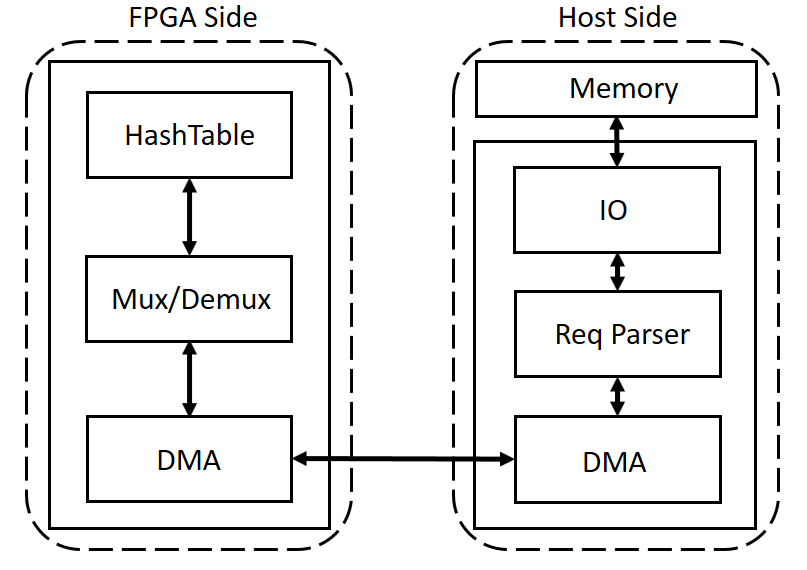
\includegraphics[width=0.6\textwidth,page=1]{scatter_gather.PNG}
		\caption{分散 - 聚集(scatter-gather)架构。}
		\label{kvdirect:fig:sg-arch}
\end{figure}


图 \ref {kvdirect:fig:scatter-gather} 表明,与CPU旁路方法相比,基于CPU的分散 - 聚集DMA的吞吐量提高了79%。
除了CPU开销之外,基于CPU的分散 - 聚集的主要缺点是额外的延迟。
为了将MMIO从CPU保存到网卡,每个门铃批量256个DMA操作,这需要 10 $\mu$s 才能完成。
使用基于CPU的分散 - 聚集网卡访问主机内存的总延迟是大约20美元,比直接DMA高出近20倍。




\begin{figure}[htbp]
	\centering
	\subfloat[读操作。\label{kvdirect:fig:sge-read}]
	{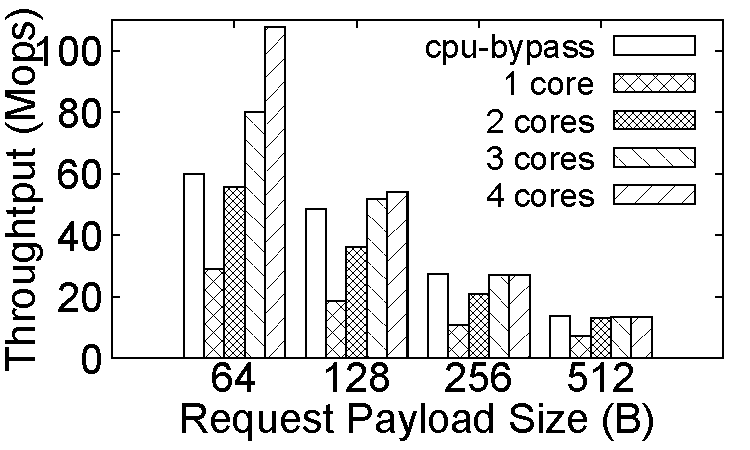
\includegraphics[width=.5\textwidth,page=1]{sg-read.pdf}}
	\subfloat[写操作。\label{kvdirect:fig:sge-write}]
	{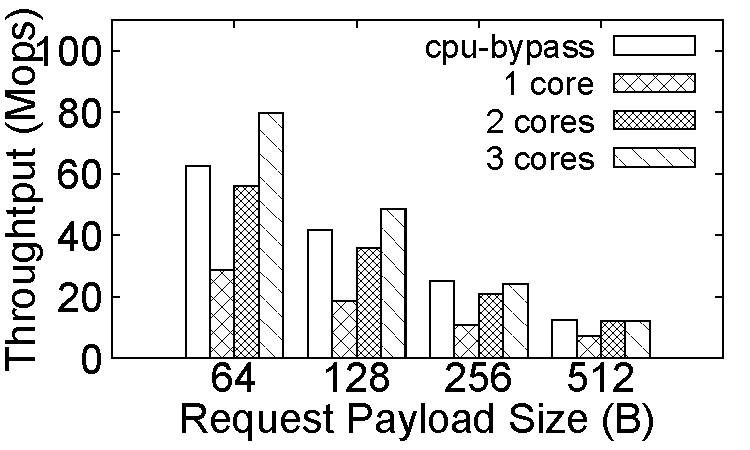
\includegraphics[width=.5\textwidth,page=1]{sg-write.pdf}}
	\caption{分散 - 聚集(scatter-gather)性能。}
	\label{kvdirect:fig:scatter-gather}
\end{figure}


\subsection{单机多网卡}
\label{kvdirect:sec:multi-nic}

KV-Direct的主要用例是启用远程直接键值访问,而无需服务器上的CPU开销。
在某些情况下,可能需要构建一个具有每服务器最大吞吐量的专用键值存储。
通过模拟,\cite {li2016full}显示了在具有四个(当前不可用的)60核CPU的单个服务器中实现十亿键值运行的可能性。
如表 \ref{kvdirect:tab:kvs-compare} 所示,在服务器上有10个KV-Direct 网卡,使用商用服务器可以轻松实现10亿键值 op/s性能。

如图 \ref{kvdirect:fig:photo},服务器消耗357瓦的功率(在墙壁上测量)以达到1.22~Gop/s GET或0.61~Gop/s PUT 的性能。


\begin{figure}[htbp]
	\centering
	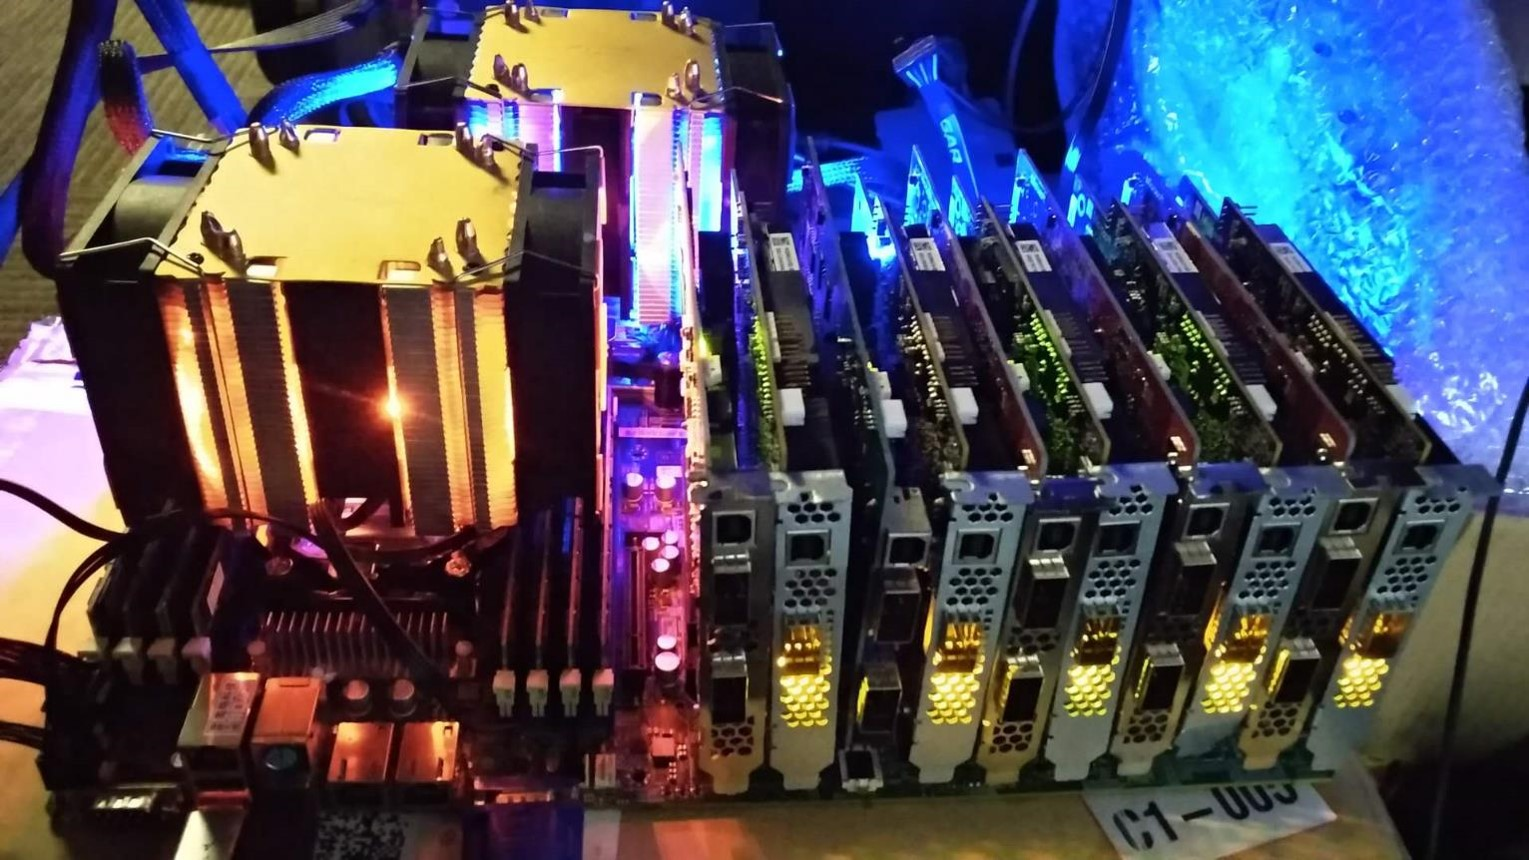
\includegraphics[width=0.9\textwidth]{figure/kvdirect_photo.jpg}
	\caption{以 357 瓦功耗实现 12.2 亿次 键值 操作每秒的 10 卡 KV-Direct 系统。}
	\label{kvdirect:fig:photo}
\end{figure}

为了使两个Xeon E5 CPU的80个PCIe Gen3通道饱和,用带有10个PCIe Gen3 x8插槽的 SuperMicro X9DRX+-F 主板替换了基准测试服务器的主板(\S\ref {kvdirect:sec:eval}) 。
使用PCIe x16到x8转换器连接每个插槽上的10个可编程网卡,每个网卡上只启用一个PCIe Gen3 x8链路,因此每个网卡的吞吐量低于图 \ref {kvdirect:fig:ycsb-tput}。
每个网卡在主机内存中拥有一个独占内存区域,并提供不相交的键分区。
多个网卡遇到与多核键值存储实现相同的负载不平衡问题。
幸运的是,对于少量分区(例如10个),负载不平衡并不重要 \cite {lim2014mica,li2016full}。在YCSB长尾工作负载下,负载最高的网卡的平均负载为1.5倍,非常流行的键所增加的负载由无序执行引擎提供(\S \ref {kvdirect:sec:ooo})。
相比之下,为了实现与240个CPU内核的匹配性能,最热 CPU 核心的负载将是平均值的10倍。
图\ref {kvdirect:fig:multiple-nics}显示KV-Direct吞吐量几乎与服务器上的网卡数量呈线性关系。


\begin{figure}[htbp]
	\centering
	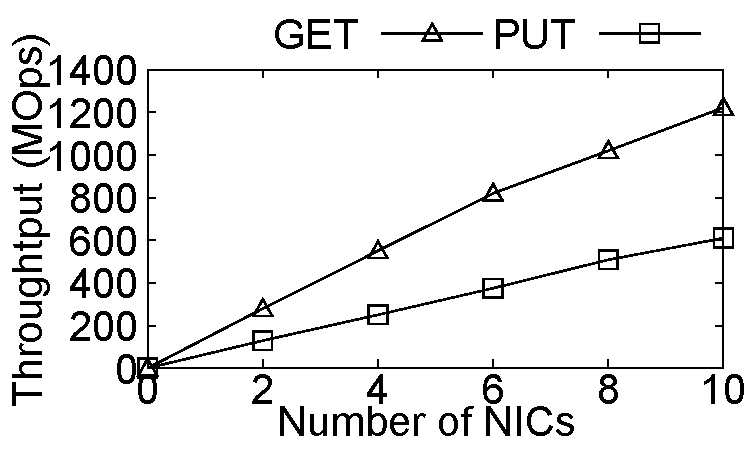
\includegraphics[width=0.5\textwidth,page=1]{multi_nic.pdf}
	\caption{单机多网卡的性能可扩放性。}
	\label{kvdirect:fig:multiple-nics}
\end{figure}


\subsection{基于 SSD 的持久化存储}

基于内存数据结构存储断电后数据会丢失。为了持久化,本节利用 SATA SSD 实现了持久化键值存储。由于服务器上的 SSD 数量是有限的,且操作系统和应用程序也运行在 SSD 上,需要对 SSD 进行虚拟化。
如图 \ref{kvdirect:fig:ssd},可编程网卡将 SSD 虚拟化成两个虚拟 AHCI HBA 设备。其中的主虚拟存储设备透明地

\begin{figure}[htbp]
	\centering
	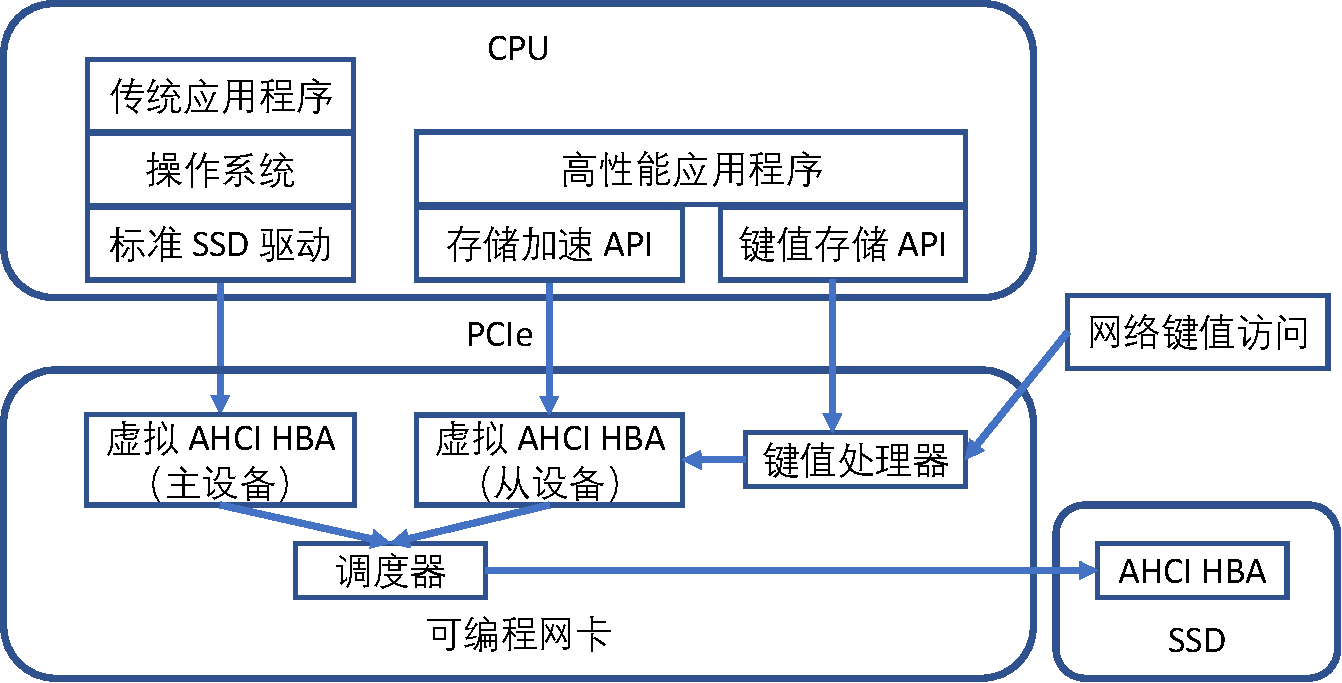
\includegraphics[width=0.9\textwidth]{ssd.pdf}
	\caption{SSD 持久化存储架构。}
	\label{kvdirect:fig:ssd}
\end{figure}



\subsection{分布式键值存储}

把键值分布到其他节点上……


\section{讨论}
\label{kvdirect:sec:discussion}

\subsection{不同容量的网卡硬件}
\label{kvdirect:sec:different-nic}

KV-Direct的目标是利用数据中心的现有硬件来卸载重要的工作负载(键值访问),而不是设计特殊的硬件来实现最大的键值存储性能。可编程网卡通常包含有限数量的DRAM用于缓冲和连接状态跟踪。 大型DRAM在芯片尺寸和功耗方面都很昂贵。

即使未来的网卡具有更快或更大的板载内存,在长尾工作负载下,本文的负载分配设计(\S \ref {kvdirect:sec:dram-cache})仍然显示出比简单的分区设计更高的性能。键统一根据网卡和主机内存容量。
表 \ref {kvdirect:tab:optimal-load-dispatch} 显示了具有10亿个键的长尾工作负载的最佳负载分配比率,不同的网卡 DRAM和PCIe吞吐率以及不同的网卡和主机比率内存大小。
如果网卡具有更快的DRAM,则将更多负载分派给网卡。负载分配比率为1表示网卡内存的行为与主机内存的高速缓存完全相同。
如果网卡具有更大的DRAM,则将稍微少量的负载分派给网卡。
如表 \ref {kvdirect:tab:optimal-load-dispatch-throughput} 所示,即使网卡 DRAM的大小只是主机内存的一小部分,吞吐量增益也很大。


\begin{table}[htbp]
	\centering
	\caption{不同网卡 DRAM / PCIe吞吐率(垂直)和网卡 /主机内存大小比(水平)下长尾工作负载的最佳负载分配比。}
	\label{kvdirect:tab:optimal-load-dispatch}
	\small
	\begin{tabular}{|l|r|r|r|r|r|r|}
		\hline
		& 1/1024 & 1/256 & 1/64 & 1/16 & 1/4 & 1 \\
		\hline
		1/2  & 0.366 & 0.358 & 0.350 & 0.342 & 0.335 & 0.327 \\
		\hline
		1    & 0.583 & 0.562 & 0.543 & 0.525 & 0.508 & 0.492 \\
		\hline
		2    & 0.830 & 0.789 & 0.752 & 0.718 & 0.687 & 0.658 \\
		\hline
		4    & 1     & 0.991 & 0.933 & 0.881 & 0.835 & 0.793 \\
		\hline
		8    & 1     & 1     & 1     & 0.995 & 0.937 & 0.885 \\
		\hline
	\end{tabular}
\end{table}


\begin{table}[htbp]
	\centering
	\caption{与简单分区相比,负载分派的相对吞吐量。行列标题与表 \ref{kvdirect:tab:optimal-load-dispatch} 相同。}
	\label{kvdirect:tab:optimal-load-dispatch-throughput}
	\small
	\begin{tabular}{|l|r|r|r|r|r|r|}
		\hline
		& 1/1024 & 1/256 & 1/64 & 1/16 & 1/4 & 1 \\
		\hline
		1/2 & 1.36	& 1.39	& 1.40	& 1.37	& 1.19	& 1.02 \\ 
		\hline
		1	& 1.71	& 1.77	& 1.81	& 1.79	& 1.57	& 1.01 \\
		\hline
		2	& 2.40	& 2.52	& 2.62	& 2.62	& 2.33	& 1.52 \\
		\hline
		4	& 3.99	& 4.02	& 4.22	& 4.27	& 3.83	& 2.52 \\
		\hline
		8	& 7.99	& 7.97	& 7.87	& 7.56	& 6.83	& 4.52 \\
		\hline
	\end{tabular}
\end{table}


乱序执行引擎(\S \ref {kvdirect:sec:ooo})可以应用于需要隐藏延迟的各种应用程序,本文希望未来的RDMA 网卡能够支持更更性能的原子操作。

在40~Gbps网络中,网络带宽限制了非批量键值吞吐量,因此本文使用客户端批处理。通过更高的网络带宽,可以减少批量大小,从而减少延迟。在200~Gbps网络中,KV-Direct网卡无需批量即可达到180~Mop/s。

KV-Direct利用广泛部署的可编程网卡和FPGA实现 \cite{putnam2014reconfigurable,caulfield2016cloud}。 FlexNIC \cite {kaufmann2015flexnic,kaufmann2016krishnamurthy} 是另一种具有可重构匹配行动表(RMT) \cite {bosshart2013forwarding} 的可编程网卡的有前途的架构。
NetCache \cite {netcache-sosp17} 在基于RMT的可编程交换机中实现键值缓存,显示了在基于RMT的网卡中构建KV-Direct的潜力。

\subsection{对现实世界应用的影响}

当KV-Direct应用于端到端应用程序时,后台计算显示了潜在的性能提升。 在PageRank \cite {page1999pagerank}中,由于每次边缘遍历都可以通过一次键值操作实现,因此KV-Direct在具有10个可编程网卡的服务器上支持1.22G TEPS。 相比之下,GRAM \cite {wu2015g}支持每台服务器250M TEPS,受交错计算和随机内存访问的约束。

KV-Direct支持用户定义的函数和向量操作(表 \ref {kvdirect:tab:kv-operations}),可以通过将客户端计算卸载到硬件来进一步优化PageRank。 类似的参数适用于参数服务器 \cite {li2014scaling}。本文希望未来的工作可以利用硬件加速的键值存储来提高分布式应用程序的性能。

\subsection{可编程网卡内的有状态处理}

本文第 \ref{chapter:clicknp} 章的 ClickNP 架构比较适合无状态或状态简单的流水线式数据包处理,而对基于连接状态或应用层请求的处理,就显得捉襟见肘。
例如,四层负载均衡器应用中的调度器和哈希表与应用逻辑耦合紧密,既不容易扩放到大量并发连接,代码的可维护性也不强。事实上在开发过程中花费了大量的时间来解决死锁问题。
为此,本章提出的有状态处理(stateful processing)和哈希表数据结构设计等基础组件可以作为很多可编程网卡应用的基础,如第 \ref{chapter:clicknp} 章的有状态网络功能(如四层负载均衡器)和第 \ref{chapter:socksdirect} 章的可扩放 RDMA。

为了模块化和可扩放性,使用 KV-Direct 作为基础后,可编程网卡上应用的架构如图 \ref{arch:fig:kvdirect_arch} 所示。
事务代表着前后依赖关系,例如有状态网络处理中的一个连接,分多个数据包的一个应用层 HTTP 请求,或者键值存储中对同一个键(key)的操作。
同一个事务中的不同请求需要依次处理,而不同事务中的请求可以并发处理。
为了隐藏延迟、最大化并发处理能力,请求调度器从基于 KV-Direct 的事务状态键值存储中查找该请求对应的事务编号,并将正在处理事务的请求排入队列。
基于 ClickNP 的数据处理流水线根据请求数据和事务状态进行处理,在处理过程中可能查询其他的数据结构(如内存分配表、主机虚拟地址映射表、防火墙规则表、路由表等)。
如果请求处理完成,响应数据进入输出重排模块,重新排列响应的顺序以满足事务处理的一致性要求(例如,不同事务的请求也要按照到达顺序依次响应),最终输出到网络。
如果请求的处理还需要依赖下一数据包或从主机内存 DMA 来的数据,为了不阻塞数据处理流水线,该请求会返回到调度器,等待依赖操作完成后再进行下一阶段的处理。


\begin{figure}[htbp]
	\centering
	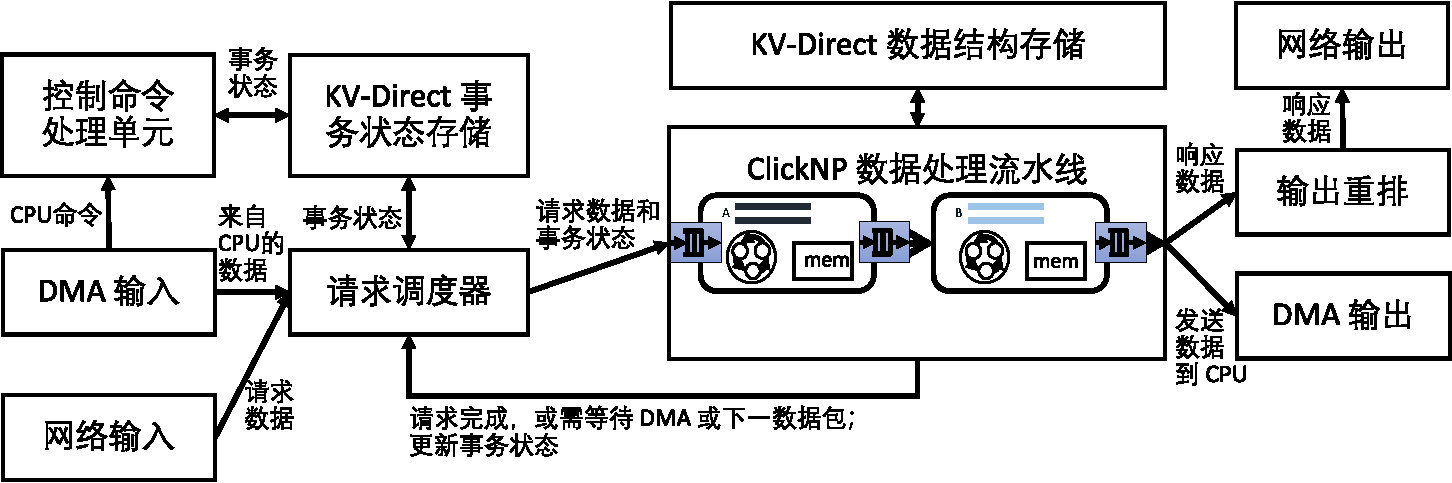
\includegraphics[width=1.0\textwidth]{../figures/kvdirect_arch.pdf}
	\caption{基于 KV-Direct 的可编程网卡应用层架构。}
	\label{arch:fig:kvdirect_arch}
\end{figure}
